\parindent=0em
\subsection{Tecnologías en realidad virtual}
\noindent

En el caso de la realidad virtual es necesario tener en cuenta otros factores para una buena experiencia aparte de la posición y orientación del usuario, como por ejemplo, la posición y gestos de las manos o la distancia interpupilar.\\

Primero de todo, hay que tener en cuenta el concepto de \textit{DoF} (del inglés Degrees of Freedom), los \textit{DoF} hacen referencia a los distintos ángulos en los que se puede mover un elemento. En los dispositivos de realidad virtual se distingue entre \textit{3DoF} y \textit{6DoF} (figura~\ref{fig:3dofvs6dof}), por ejemplo, en un dispositivo con \textit{3DoF}, solo se tiene en cuenta la rotación mientras que si posee \textit{6DoF} se tiene en cuenta estas 3 rotaciones y el movimiento del dispositivo en 3 ejes.\\

\begin{figure}[H]
    \centering
    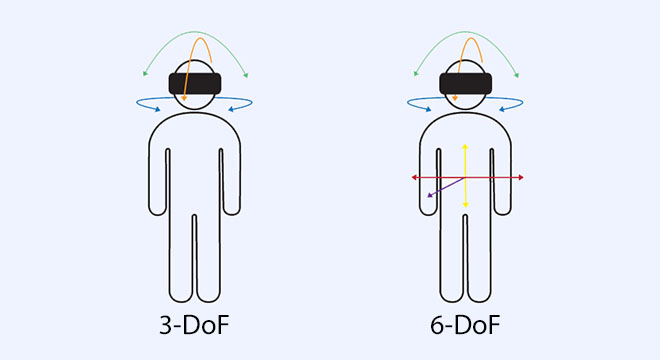
\includegraphics[scale=0.6]{Images/Estado del arte/3dofvs6dof.jpg}
    \caption{Diferenciación entre \textit{3DoF} y \textit{6DoF}.}
    \label{fig:3dofvs6dof}
\end{figure}

%https://virtualspeech.com/blog/degrees-of-freedom-vr


Del mismo modo, el \textit{DoF} está relacionado con el \textit{hand tracking} o seguimiento de manos, un proceso mediante el cual se obtiene la posición de las manos y también, los gestos que están realizando como cerrar el puño o agarrar algo, entre otros. Un modelo que se presenta para hacer este seguimiento~\cite{robustHandTracking} habla de la dificultad del proceso debido a la gran cantidad y variación de \textit{DoF} que pueden tomar las manos. Este modelo se basa en una única cámara de profundidad mediante la cual obtienen imágenes que luego procesan utilizando aprendizaje automático para finalmente poder obtener la posición de las manos y su rotación en tiempo real.\\

Aunque actualmente no es obligatorio para un correcto funcionamiento de la realidad virtual que los dispositivos utilicen \textit{hand tracking} (ya que se puede utilizar un par de mandos en su lugar) es un factor que incrementa la inmersión del usuario notablemente, asimismo, no es obligatorio el uso de \textit{eye tracking} o seguimiento de ojos pero puede ser beneficioso para la experiencia. Gracias al \textit{eye tracking} se puede obtener información útil ~\cite{eyetrackingVR} como las regiones de interés del espacio 3D y saber en qué momento se ha mirado hacia estas regiones, también, se puede cambiar la información en pantalla basándose en dónde está mirando el usuario o incluso controlar las interfaces virtuales con la mirada.\\

Como se ha mencionado anteriormente, la distancia interpupilar o \textit{IPD} (del inglés interpupillary distance) es otro factor a tener en cuenta a la hora de una experiencia virtual satisfactoria. La \textit{IPD} es la distancia (normalmente medida en milímetros) entre los centros de los dos ojos (figura~\ref{fig:IPDExample}).

\begin{figure}[H]
    \centering
    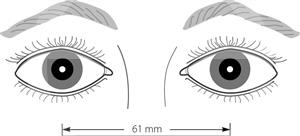
\includegraphics[scale=1]{Images/Estado del arte/IPD.jpg}
    \caption{Medición de la distancia interpupilar.}
    \label{fig:IPDExample}
\end{figure}

Según un estudio realizado con distintas personas haciendo variaciones del \textit{IPD}~\cite{IPDTest} en un \textit{HMD} (del inglés head mounted display) o casco de realidad virtual, se llegó a la conclusión de que no había alteraciones a la hora de distinguir los tamaños de los objetos virtuales o afectaciones en la claridad de la visión, en cambio, los usuarios notaron una mayor fatiga con una configuración en el \textit{HMD} de 50 mm y 74 mm en la distancia interpupilar en comparación a un valor del \textit{IPD} adecuado a su distancia interpupilar anatómica.
%https://www.aao.org/image/interpupillary-distance-2




